\documentclass{article}
\usepackage[utf8]{inputenc}
\usepackage{amsmath}
\usepackage{graphicx}
\usepackage{float}
\graphicspath{ {./Figures/} } 

% ========== Title Page ==========
\title{Heat Pump Lab}
\author{
	\textbf{Submitted by}: \\
	Henry V. Gilbert \\
	The University of Tennessee Knoxville \\
	hgilber1@vols.utk.edu \\
	(931) - 335 - 0669 \\
	960 Riverside Forest Way
	Apt. 002 \\
	Knoxville TN, 37915\\ \\ \\ \\ \\ \\ \\ 
	\textbf{Submitted to: }\\ 
	Dr. Seyedreza Djeddi \\
	Research Assistant Professor and Lecturer \\
	Tickle College of Engineering, MABE Department \\
	314 Perkins Hall \\
	1506 Middle Drive \\
	Knoxville TN, 37996 \\
	}
\date {March 12 2019}

\begin{document}
\maketitle

% ========== Intro Section  ==========
\newpage
\section{Introduction}
\paragraph{Background} 
The vapor-compression refrigeration cycle has been considered a modern masterpiece of engineering. Having the ability
to manipulate properties based on simple engineering principles has had insurmountable implications in the industry. 
Found in HVAC systems for homes and buildings, engine cooling systems, and even computer cooling, this work of 
art is one of the most prolific inventions in modern engineering.

The refrigeration cycle works on two basic principles. 1: Compressing a gas increases its temperature, and expanding a gas decreases its temperature. 2: Energy naturally flows from high temperature to lower temperature. Using these two principles, a refrigeration cycle can be constructed with four main components: compressor, condenser, throttle valve, and evaporator. The compressor required a work input to compress a refrigerant vapor, thus increasing its pressure and temperature into a superheated vapor. This superheated vapor enters a condenser where it expells heat at a constant pressure into the environment, thus causing the previously superheated vapor to "condense" into a high pressure liquid around saturation temperature, where it enters the throttling valve. This low temperature high pressure liquid expands isenthalpically and acts as an inverse of the compressor, where the pressure is significantly reduced, causing the temperature of the refrigerant to drop into a subcooled state. This subcooled and low pressure liquid enters the evaporator where it absorbs heat from the environment and cools the ambient air. The evaporator allows the subcooled liquid to absorb enough heat that it begins to evaporate and turn into a low pressure superheated vapor, which enters the compressor and starts the cycle over again. 

\begin{figure} [H]
	\centering
	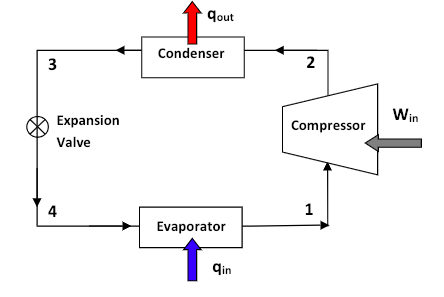
\includegraphics[width=0.6\textwidth]{Vapor_comp_cycle}
	\caption{\textbf{Diagram of the Idealized Vapor Compression Cycle}}
\end{figure}

	
\paragraph{Objectives}
% Determine COPc, COPh, efficiency, for water and air evaporator mode. 
% Determine refrigerant superheat and subcooling
% Draw the phases on a P-h diagram
% Compare air vs water modes for evaporator heat exchanger 
The objectives for this experiment were to take measurements from the heat pump and to use those measurements to calculate performance data (coefficient of performance and compressor efficiency). Using CoolProp, a Python program for determining refrigerant properties, enthalpy values were obtained for each refrigerant state in the cycle. Additionally, specific heats and saturation properties  were determined. With these values, the superheat, subcooling, and quality of the refrigerant were calculated. Afterwards, the refrigeration cycle was plotted on a P-h diagram. 

% ========== Methodology ==========
\section{Methodology}
\paragraph {Apparatus}
\begin{figure} [H]
	\centering
	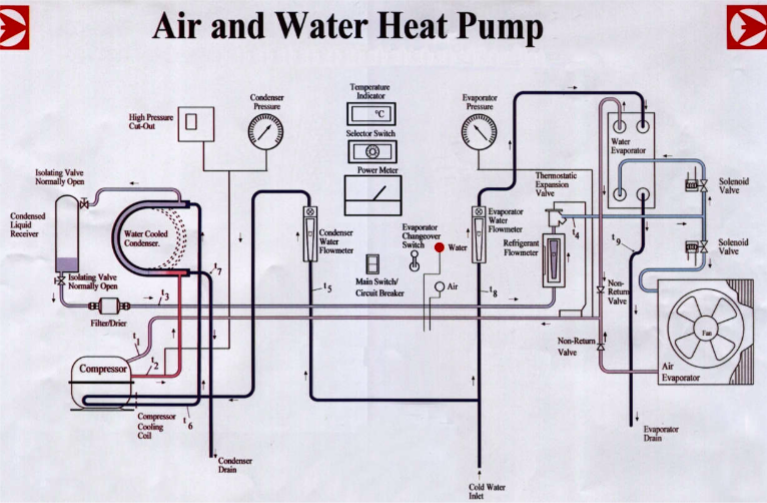
\includegraphics[width=0.9\textwidth]{hylton_diagram}
	\caption{\textbf{Schematic of the Heat Pump}}
\end{figure}
This system involves using the "Hylton Air and Water Heat Pump System." % Show schematic and picture.
The configuration has 8 key thermocouples, three flow rotameters, and two onboard pressure gages. The first four thermocouples are placed at the compressor, condenser, throttle valve, and evaporator (named T1, T2, T3, and T4 in the experiment, respectively). Temperatures 6 and 7 correspond to the condenser inlet and outlet, and temperatures 8 and 9 correspond to the evaporator inlet and exit. The three rotameters measure the refrigerant flow rate, the condenser water flow rate, and the evaporator water flow rate. Onboard pressure gages were used to determine the high side and low side pressure of the system. With this configuration, the condenser will only exchange heat with a waterstream. This different from a home heating system, where the heat is exchanged into ambient air. This apparatus features two evaporator modes: water cooling and air cooling. Water cooling mode allows the evaporator to exchange heat with a water stream, and air cooling mode allows the cooled refrigerant to exchange heat with ambient air. Home systems work similarly to air evaporator mode, while water heaters and engine coolants work with water cooling mode. 
 
\paragraph{Test Procedure}
% Show energy balances 
First, the main water valve was turned on and set the heat pump to water evaporator mode. The condenser water flow was set to 30 $ \frac{g}{s} $, and the evaporator flow was set to 45 $ \frac{g}{s} $. Check to ensure that no bubbles were present in the refrigerant flow meter. Since the pressures in the experiment must be absolute, the ambient pressure was recorded and subsequently added to each gage pressure reading.  Once the system had been given ample time to reach a stable state (around 5-10 mins), the rotating temperature knob was turned from settings 1-9 (corresponding to temperatures in Figure 1) and the temperatures were recorded. The high side pressure, low side pressure, refrigerant flow, power, condenser flow rate, and evaporator flow rate were recorded. Once all measurements were recorded, the heat pump was switched into air evaporator mode, and the above measurements were taken again. Additionally, the ambient air temperature was recorded using a dry bulb thermometer. 

% ======================= Data analysis section. ========================
\paragraph{Data Analysis}

Performance values were obtained from energy balances. On the condenser and evaporator, refrigerant and (water or air) is entering and exiting the system in steady state. For the condenser, the energy balance is as follows: 
\begin{figure} [H]
	\centering
	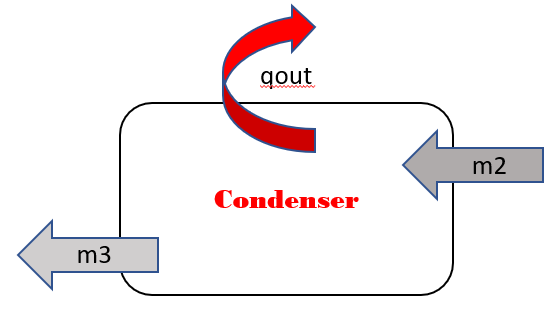
\includegraphics[width=0.9\textwidth]{ebal_condenser}
	\caption{\textbf{Energy Balance for Condenser}}
\end{figure}
Here, $\dot{m_2}$ and $\dot{m_3}$  represent the refrigerant inlet and outlet of the condenser, respectively. Based on the energy balance, $q_{out} = \dot{m} (h_3 - h_2) $. The heat leaving the condenser represents the heat supplied to the user during heating mode. Therefore, $$ COP_H = \frac{Q_{out}}{W_{in}} = \dot{m}_{ref} \times \frac{h_2 - h_3}{W_{in}} $$ \\
$Q_{out}$ is absorbed directly by a water stream. The amount of heat absorbed by the water stream can be calculated using:
$$ Q_{into water} = \dot{m} \Delta{H} = \dot{m} \times C_p \times \Delta T  $$
Ideally, the value of $Q_{out}$ from the refrigerant should be identical to $Q_{in}$ to the water. The ratio of $\frac{Q_{out}}{Q_{in}}$ checks the validity of the heat exchanged between the water and refrigerant. A value of 1.00 means that excatly all the heat from the refrigerant is transferred perfrectly to the water. 

During cooling mode, the evaporator absorbs heat from the ambient air and cools the room. The refrigerant energy balance for the evaporator is as follows: 
\begin{figure} [H]
	\centering
	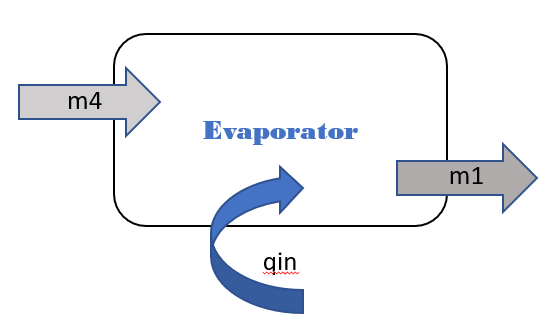
\includegraphics[width=0.9\textwidth]{ebal_evap}
	\caption{\textbf{Refrigerant energy balance on the evaporator}}
\end{figure}
Based on this energy balance, $\dot{m_4}$ and $\dot{m_1}$ correspond to the refrigerant entering and leaving the evaporator, respectively, and is derived as $q_{in} = \dot{m} (h_1 - h_4) $. Therefore, for cooling mode, the performance is determined from $$ COP_C = \frac{Q_{in}}{W_{in}} = \dot{m}_{ref} \times \frac{h_1 - h_4}{W_{in}} $$ 

$Q_{in}$ is transferred from water during water evaporator mode and from air during air evaporator mode. In air evaporator mode, the calculations for the condenser are the same. However, for the evaporator, the work input into the compressor is not directly known since the power input is split between the compressor and the evaporator fan. Assuming that the compressor operates with the same isentropic efficiency, the work input can be estimated using 
$$ \dot{W_{in}} = \frac{\dot{m} (h_2 - h_1)} {\eta} $$ 
The calculations for $COP_H$ and $COP_C$ are the same for air evaporator mode. 

The goal of the compressor is to compress the refrigerant vapor and increase the temperature and pressure. The compressors isentropic efficiency is based on the ratio of the heat added to the vapor compared to the work input into the compressor, shown as $$ \eta =  \dot{m}_{ref} \times \frac{h_2 - h_1}{W_{in}} $$ 

Superheat, subcooling, and quality values can be obtained for each trial using the following formulas:
$$ Superheat = T - T_{Sat} = T_{Compressor} - T_{Sat @ Tcomp} $$
$$ Subcooling = T_{Sat} - T_{Throttle}  $$
$$ Quality = \frac{H_{Throttle}- H_{TSat @ Throttle}}{H_g - H_f} $$


% ========== Results ==========
\newpage
\section{Results and Discussion}\label{conclusions}
\paragraph {Results}
First shown is the results for the water mode condenser. Results were taken from trial run 5.  

% Data for the water run. Ref, condenser, and evap. 
\begin{figure} [H]
	\centering
	\includegraphics[width=0.8\textwidth]{W_run}
	\caption{\textbf{Heat Pump Data for Water Run}}
\end{figure}

\begin{figure} [H]
	\centering
	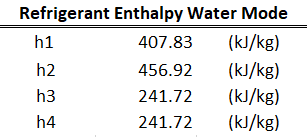
\includegraphics[width=0.6\textwidth]{W_enthalpy}
	\caption{\textbf{Refrigerant enthalpy for water run. Calculated using CoolProp}}
\end{figure}

\begin{figure} [H]
	\centering
	\includegraphics[width=0.8\textwidth]{W_performance}
	\caption{\textbf{Performance data for water cooling mode}}
\end{figure}
The specific heats were calculated using CoolProp at the desired temperature. $Q_W$ and $Q_H$/$Q_C$ were derived using theoretical energy balances on the condenser and evaporator. Coefficients of performance were calculated using energy balances. 

\begin{figure} [H]
	\centering
	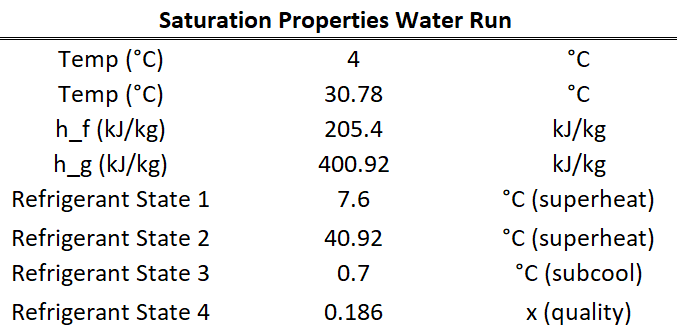
\includegraphics[width=0.74\textwidth]{W_saturationProps}
	\caption{\textbf{Saturation properties for refrigerant in water mode}}
\end{figure}

\begin{figure} [H]
	\centering
	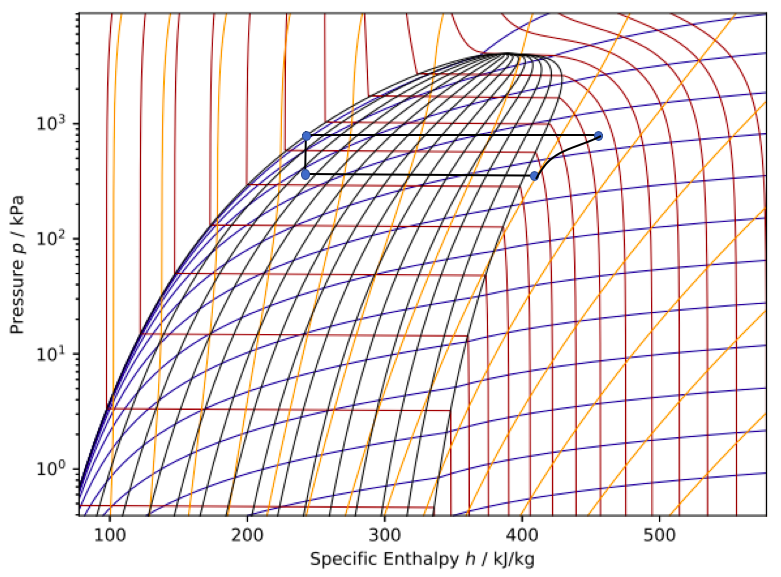
\includegraphics[width=0.75\textwidth]{ph_water}
	\caption{\textbf{P-h Diagram for water evaporator run}}
\end{figure}

\begin{table} [H]
	\centering
	\caption{\textbf{P-h diagram points water}}
	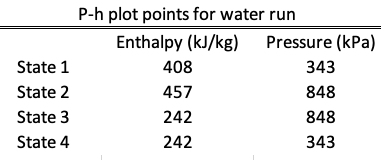
\includegraphics[width=0.55\textwidth]{ph_points_water}
\end{table}

\newpage
\paragraph{Air Evaporator Mode}
Below are the results for the air evaporator mode. This mode used air to exchange heat with the evaporator instead of water. Therefore, $Q_W$ measurements  and specific heat properties were not taken. 
\begin{figure} [H]
	\centering
	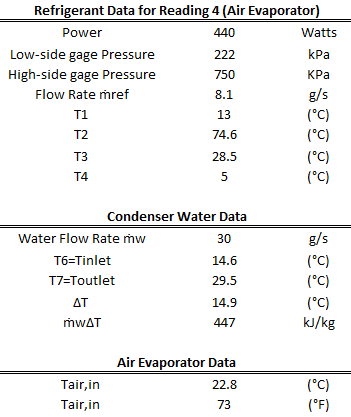
\includegraphics[width=0.9\textwidth]{A_run}
	\caption{\textbf{Heat pump data for air evaporator run}}
\end{figure}


\begin{figure} [H]
	\centering
	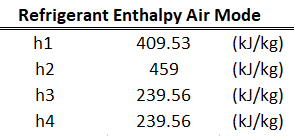
\includegraphics[width=0.6\textwidth]{air_enthalpy}
	\caption{\textbf{Enthalpy properties for air evaporator mode. Calculated using CoolProp}}
\end{figure}

\begin{figure} [H]
	\centering
	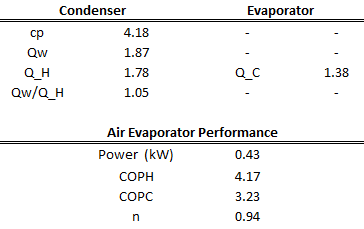
\includegraphics[width=0.9\textwidth]{air_performance}
	\caption{\textbf{Performance data for air run}}
\end{figure}
Power output was determined using the isentropic efficiency from the water evaporator mode. 

\begin{figure} [H]
	\centering
	\includegraphics[width=0.70\textwidth]{A_saturation}
	\caption{\textbf{Saturation properties for air evaporator run}}
\end{figure}

\begin{figure} [H]
	\centering
	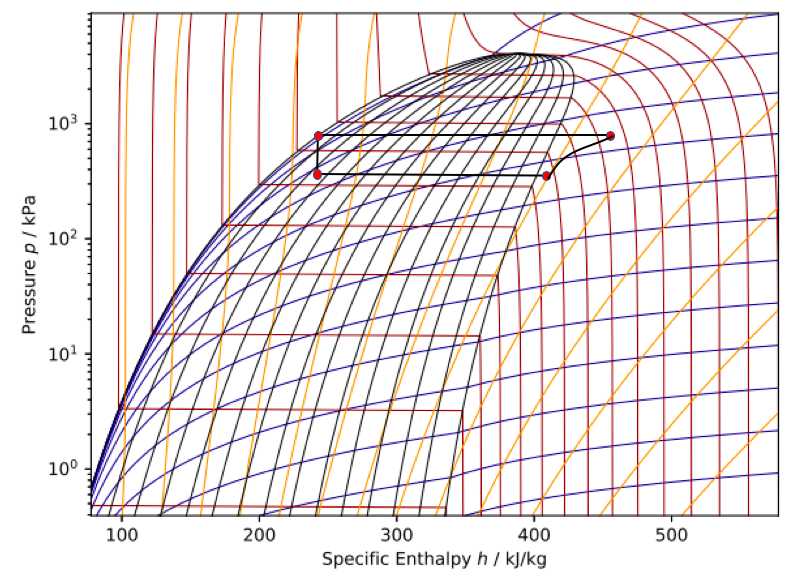
\includegraphics[width=0.75\textwidth]{ph_air}
	\caption{\textbf{P-h Diagram for water evaporator run}}
\end{figure}

\begin{table} [H]
	\centering
	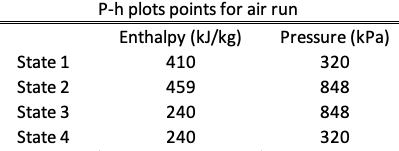
\includegraphics[width=0.7\textwidth]{ph_points_air}
	\caption{\textbf{P-h diagram points Air}}
\end{table}


\begin{figure} [H]
	\centering
	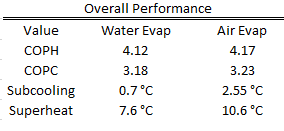
\includegraphics[width=0.7\textwidth]{overall_perform}
	\caption{\textbf{Performance comparison between air and water evaporator}}
\end{figure}

% ========== Discussion section  ==========
\section {Conclusions and Recommendations}
From the data, it is shown that the performance during air mode was better than water mode. Both coefficients of performance were higher during air evaporator mode, and more subcooling and superheat was obtained using air mode. These values are based on the assumption that the isentropic efficiency remained the same during both runs. Water has a much high specific heat than air. This means that based on the molecular composition, it requires more energy to heat the same amount of water compared to air. Because of this, water in the evaporator has a harder time giving off its heat to the refrigerant during cooling. This has a compounding effect on on the compressor as well. Performance of the cycle tends to increase with an increase in superheat. This is because the compressor has to work less to compress the vapor into a superheated state. The superheat from the evaporator gives the compressor a little boost in its job. Because the water can not exchange heat with the refrigerant as well as air, the temperature of the refrigerant leaving the evaproator tends to be lower when it enters the compressor. Comparatively, this means that the superheat for water mode will be lower than with air mode, and was demonstrated in Figure 13. 

Air and water evaporator modes differ in both their performance and requirements. Homes need a mix of both. Enjoying ice makers is a result of the evaporator cooling a liquid, and staying cool during the summer is a result of the evaporator cooling air. Both vary based on the needs of the user. 

Some implications in the experiment could have caused slight mistakes in data. Since the water system was hooked up into Dougherty's plumbing system, random change in water pressure (flushing toilets, washing hands, etc.) might have caused variations in the water flow rates. The compressor does have a heat return system, but the energy balances in the experiment never took into consideration the heat lost from the compressor, which was pressent because the compressor was naturally warm during operation. If the compressor was perfectly insulated, there would be no heat lost to the ambient air during compression. 

% ========== Appendices ==========
\end{document}
